\documentclass[a4paper]{report}
% Packages and global settings here
\usepackage{graphicx}
\usepackage{hyperref}
\usepackage{amsmath}
\usepackage[backend=biber, style=ieee]{biblatex}
\usepackage{float}
\usepackage[T1]{fontenc}


\hypersetup{							% Information sur le document
pdfauthor = {Gatien CHENU,
			Leon WAGNER,
			Inas ZAMANI,},			% Auteurs
pdftitle = {Multimodal product data classification},			% Titre du document
pdfsubject = {Project Report},		% Sujet
pdfkeywords = {Tag1, Tag2, Tag3, ...},	% Mots-clefs
pdfstartview={FitH}}					% ajuste la page à la largueur de l'écran


%régler l'espacement entre les lignes
\newcommand{\HRule}{\rule{\linewidth}{0.5mm}}

%page de garde
\addbibresource{sources.bib}	
\graphicspath{ {./images/} }

	

\title{\LARGE{"Multimodal product data classification"}}
\date{\today}

\begin{document}
\pagenumbering{gobble} %disable page numbers

% Include the start page

	\begin{titlepage}
		\centering
		\vspace*{1cm}
		\Huge
		\textbf{Multimodal product data classification}
		
		\vspace{0.5cm}
		\LARGE
		%Subtitle or Additional Information
		
		\vspace{1.5cm}
		
		\textbf{Names}
		
		\vfill
		
		%Text
		
		\vspace{0.8cm}
		
		\Large
		Ateliers d'apprentissage automatique\\
		Université de Strasbourg\\
		January 26, 2024
	\end{titlepage}


\pagenumbering{roman} % set page numbering to roman
\tableofcontents
\newpage

\pagenumbering{arabic} % set page numbering to arabic and start from 1
% Include the introduction
\chapter{Introduction}
\label{sec:introduction}

The advancement of e-commerce has brought with it a myriad of opportunities and challenges, particularly in the realm of product cataloging and classification. As online marketplaces expand, the task of efficiently categorizing a vast number of products becomes increasingly complex and critical. This challenge is exemplified in the case of Rakuten, a global leader in e-commerce, known for its expansive marketplace that hosts a diverse range of products.

Rakuten, founded in Japan in 1997, revolutionized online shopping with its marketplace concept and has since grown into a major e-commerce platform \cite{brian-2022}. It boasts a community of over 1.3 billion members \cite{statista-2023} and a wide array of services including communications, financial services, and digital content. The Rakuten Institute of Technology (RIT), serving as its research and innovation arm, focuses on areas like computer vision, natural language processing, and human-computer interaction to enhance and innovate within the e-commerce space.

This report addresses a specific challenge posed by Rakuten France: the large-scale multimodal (text and image) classification of products into predefined type codes. In an online marketplace, products are typically accompanied by titles, descriptions, and images. The classification of these products into correct categories is crucial for various aspects of e-commerce, such as personalized recommendations, search optimization, and efficient query processing. However, the task is not straightforward due to the sheer volume of products, the variety of classes, and the common issue of unbalanced data distributions in large catalogs.

The primary objective of this challenge is to develop a model capable of accurately categorizing products based on their textual and visual information. This involves predicting the appropriate product type code for each item in Rakuten France's catalog, a task that requires an intricate understanding of both the textual and visual characteristics of the products. The complexity of this challenge is heightened by the intrinsic variability and potential inconsistencies in product labels and images.

To facilitate this endeavor, Rakuten France has provided a dataset comprising approximately 99,000 product listings in a CSV format, which includes both training and test sets. The dataset contains product titles, detailed descriptions, images, and corresponding product type codes. The benchmark for this challenge is the weighted-F1 score, a metric that balances precision and recall, and is particularly useful in scenarios with uneven class distributions \cite{10.1093/mnrasl/slac120}.

In summary, this report delves into the development of a multimodal classification system for Rakuten's extensive product catalog. The focus is on leveraging both textual and visual data to achieve accurate and efficient product categorization, a task essential for enhancing the user experience and operational efficiency in the dynamic world of e-commerce.

%\subsection{Background}
%\label{subsec:background}
%Sentence here. % Template text for the Background subsection.

%\subsection{Motivation}
%\label{subsec:motivation}
%Sentence here. % Template text for the Motivation subsection.

%\subsection{Aim and Objectives}
%\label{subsec:aims}
%Sentence here. % Template text for the Aim and Objectives subsection.

%\subsection{Scope}
%\label{subsec:scope}
%Sentence here. % Template text for the Scope subsection.

%\subsection{Document Structure}
%\label{subsec:structure}
%Sentence here. % Template text for the Document Structure subsection.

% Main content starts
\chapter{Data exploration}


\section{The datasets}
Rakuten France provided a dataset consisting of approximately 99 000 product listings in CSV format. This dataset includes both the training set with 84 916 entries and the test set with 13 812 entries. Each entry comprises product designations, product descriptions, product images, and their corresponding product type code.

The datasets are organized based on two criteria: training or test and input or output. The data is available in three distinct csv files:

\begin{enumerate}
    \item X train.csv: Training input file
    \item Y train.csv: Training output file
    \item X test.csv: Test input file
\end{enumerate}

The images.zip file contains all the images. Extracting this file results in a folder named "images" with two subfolders, "image training" and "image test," containing training and test images, respectively.

\subsection{X train.csv}
The input files follow the common CSV format, where the first line serves as the header, and columns are delimited by commas. The columns in these files include an integer ID for product identification, a product designation providing a concise product summary, a more detailed product description (which may contain NaN values for products lacking this information), a unique product ID (productid), and a unique image ID (imageid).

\subsection{Y train.csv}
Turning attention to Y train, it contains two columns : an integer ID for product identification and the product type code.

\subsection{Y test.csv}
The X test table mirrors the structure of X train, serving as a dataset for Rakuten to assess the performance of the chosen model. With 84,916 observations or products and four variables, X test reflects the same information as X train

\section{Data visualization}
In an effort to comprehend the dataset's composition before visualization, it was imperative to explore its structure and understand the distribution of key attributes.\\

\subsection{Columns composition}
First of all, there are several empty values in the description column, which means that not all products are uploaded with a description. \\


\begin{figure}[h]
    \centering
    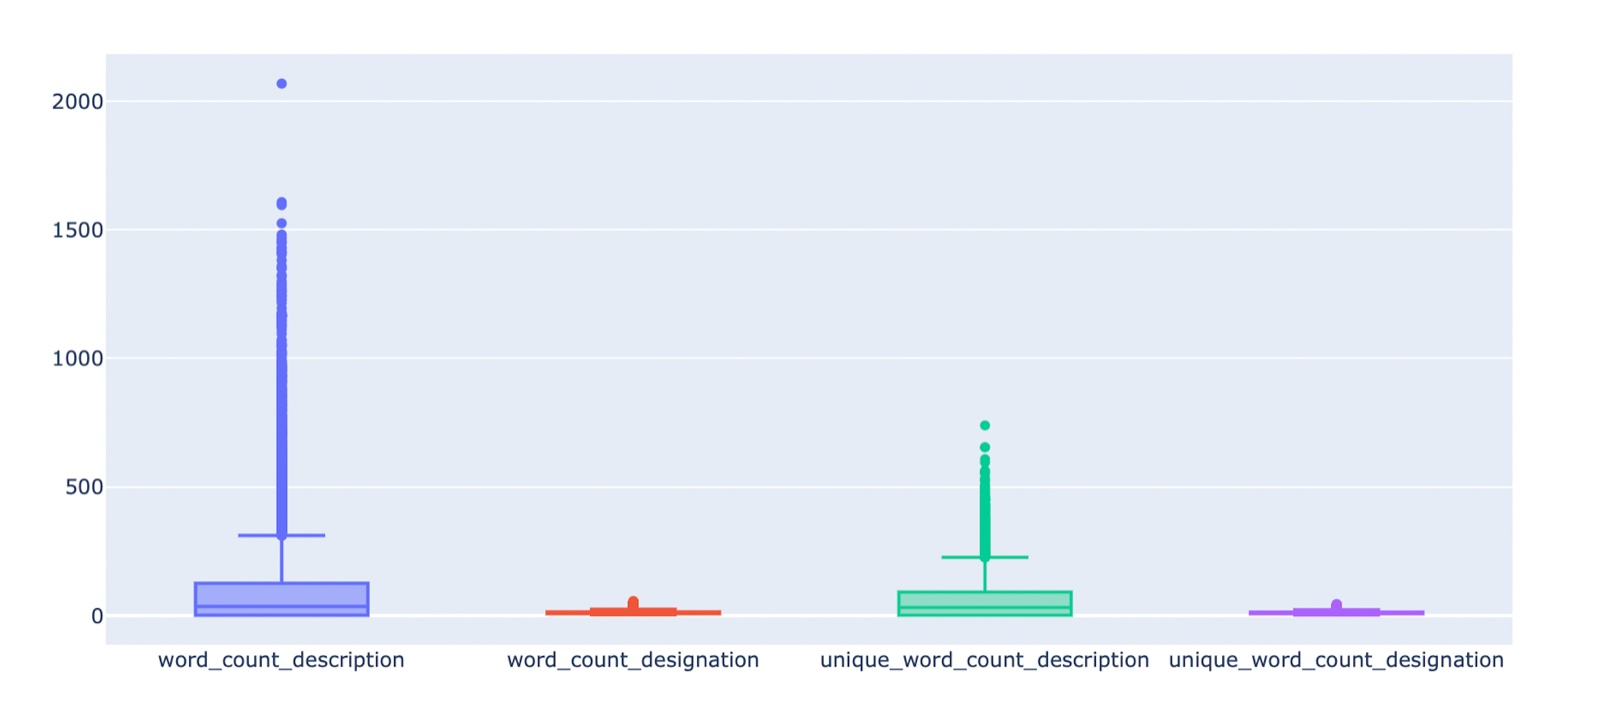
\includegraphics[width=1\textwidth]{word_count.jpeg}
    \caption{Word Counts for Both Designation and Description.}
    \label{fig:word_count}
\end{figure}

The graph shows that despite the significant difference between the word count for description and that of designation, that same difference isn't as important for the unique word count. \\
This comparison between the "description" and "designation" variables indicates that the "description" column likely contains a significant amount of information, despite the presence of a substantial number of NaNs (missing values). Therefore, we should refrain from removing this column during the handling of missing values. We will take that into consideration while coding our model. Some inputs will have more furnished features than others. \\

\subsection{Product categories}
Moreover, it is revealed that all products in X train have been categorized into 27 different product types, each identified by a unique numeric code. The dataset exhibits a light imbalance due to varying observation counts across these categories.
The following graphics demonstrate that : \\

\newpage

\begin{figure}[h]
    \centering
    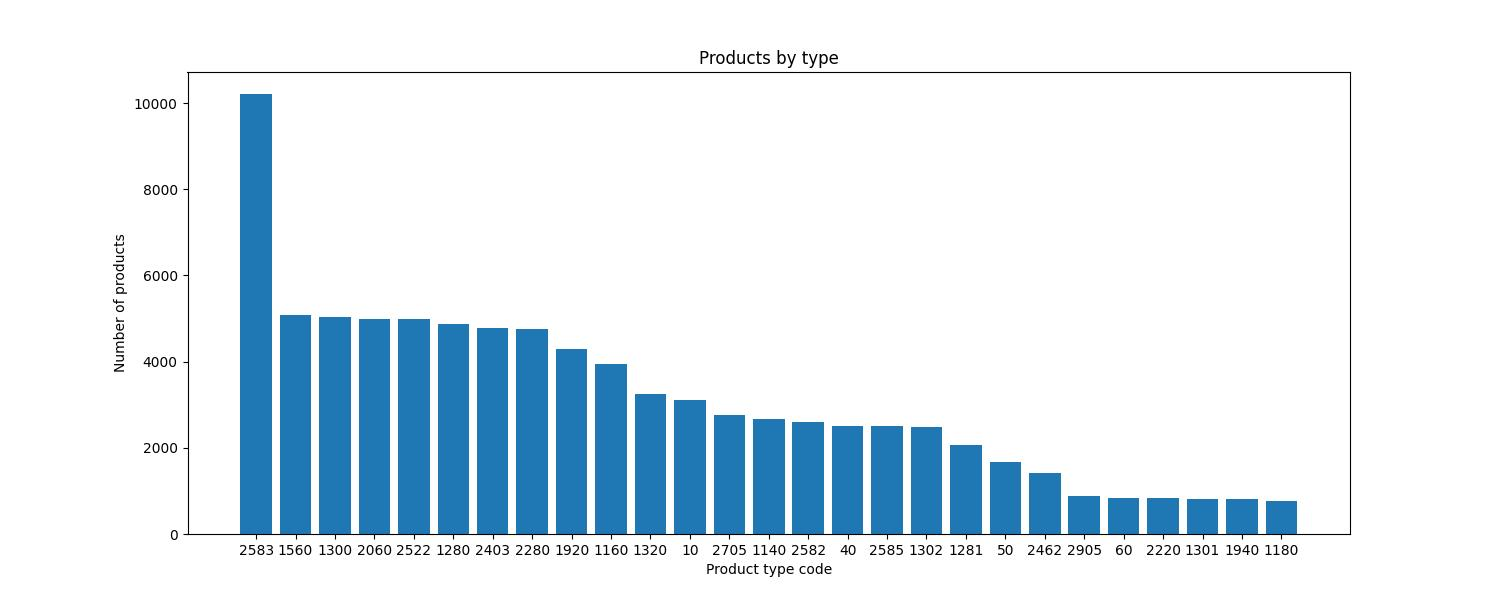
\includegraphics[width=1\textwidth]{bar_plot.jpeg}
    \caption{Number of products per category.}
    \label{fig:nproduct}
\end{figure}


To see how different product types are distributed, we can use a pie chart. \\

\begin{figure}[h]
    \centering
    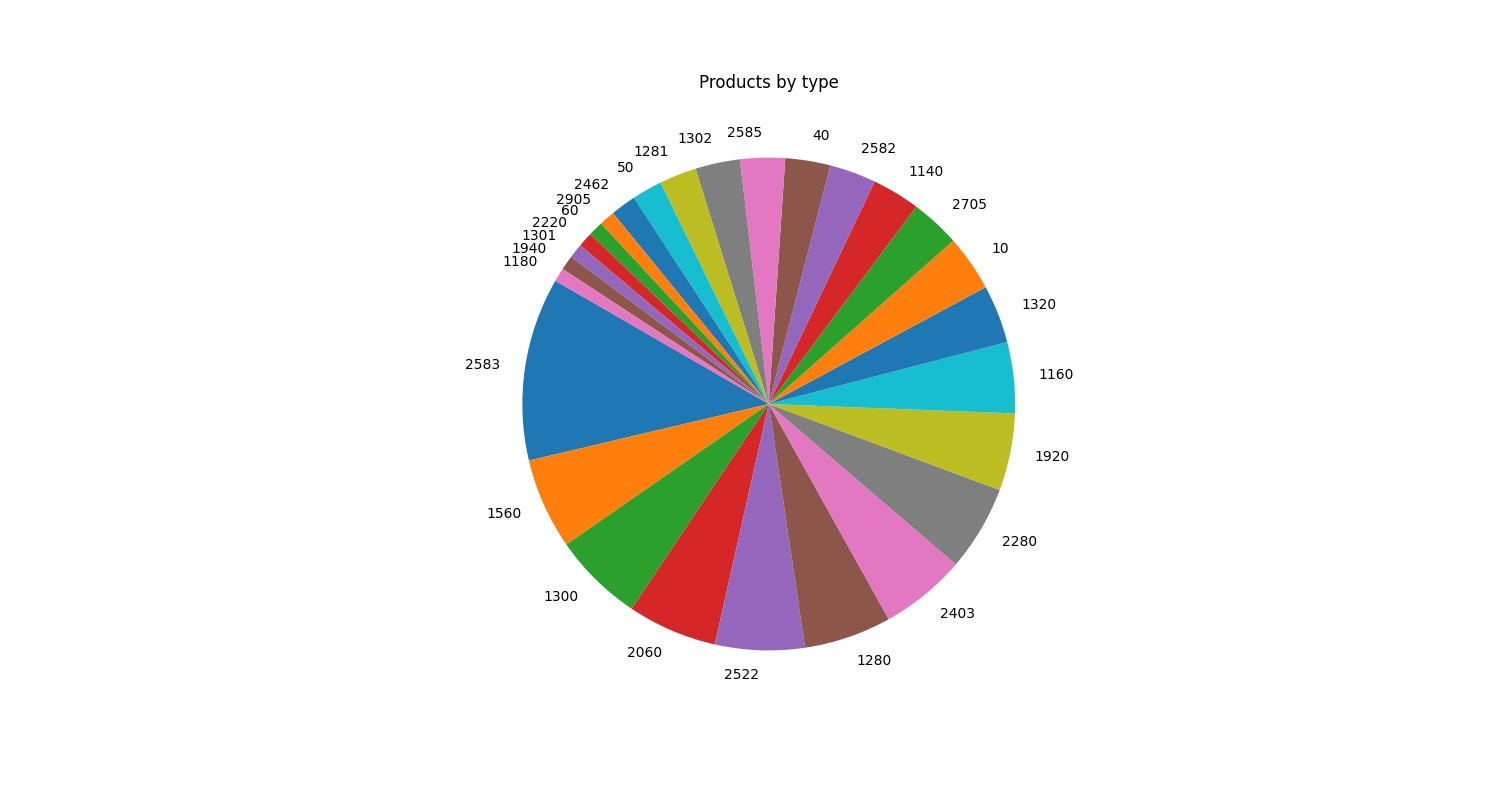
\includegraphics[width=1\textwidth]{pie_plot.jpeg}
    \caption{Distribution of products per category}
    \label{fig:product}
\end{figure}


We can see that category '2583' contributes significantly to the whole compared to other categories.On the other hand, the categories with the smallest number of samples will be more challenging to detect. We have an unbalanced dataset as the number of observations is not the same for all categories. This should be taken into account during modeling.

\newpage
\subsection{U-map}

As the UMAP algorithm takes numerical input, certain modifications were applied to the "designation" column to facilitate its integration into the analysis:  the code we have on the notebook systematically cleans the text by removing digits, punctuation, diacritics, HTML tags, and URLs. The text is then converted to lowercase, tokenized using NLTK's word tokenizer, and further processed with Keras Tokenizer, which filters out specified characters. Additionally, the sequences of tokenized words are padded using Keras' pad sequences function to ensure uniform length. Two new columns, 'designation sequences' and 'designation padded', are created in the DataFrame to store the intermediate and final processed text, making it suitable for subsequent analysis or machine learning tasks. \\

A UMAP plot was generated to explore the underlying structure of the dataset. The plot revealed distinct clusters, some of which were readily identifiable, while others appeared less defined. Outliers were also observed, indicating certain products or groups of products that deviate significantly from the main clusters.



\section{Method}
\label{sec:method}

\subsection{Data Preparation}

\subsection{Visualisation}

\subsection{Feature Extraction}

\subsection{Modelling}

\subsubsection{Integrating CLIP for Enhanced Multimodal Product Classification}
Central to our approach is the integration of OpenAI's CLIP (Contrastive Language–Image Pretraining) model. CLIP embodies a novel paradigm in artificial intelligence, harmonizing the interpretation of visual and textual data through a multimodal learning framework.

CLIP operates on a dual-encoder structure, comprising an image encoder and a text encoder. This architecture is instrumental in processing and correlating visual and textual inputs. The model's training utilizes a contrastive learning method, where it is exposed to numerous images and their corresponding textual descriptions, drawing from a diverse and extensive internet-sourced dataset. This training enables CLIP to develop a nuanced understanding of the intricate relationships between text and images.

In the realm of product classification, CLIP's integration offers a transformative potential. Our model leverages CLIP's proficiency in associating product images with their textual descriptions, such as titles and detailed narratives. This synergy allows for a more nuanced and accurate classification of products into their respective categories.


\subsection{Evaluation}

\chapter{Evaluation}
\label{sec:evaluation}
\section{Comparison of different models} 

\begin{equation}
	F1 = \frac{2 \times \text{TP}}{2 \times \text{TP} + \text{FN} + \text{FP}}
\end{equation}

The F1 score is a statistical measure used to evaluate the precision and recall of a model's predictions, essentially capturing the balance between the model's accuracy and its comprehensiveness in identifying relevant instances. Precision represents the accuracy of positive predictions, while recall measures the model's ability to identify all actual positive instances. The F1 score is the harmonic mean of precision and recall, thus ensuring that both metrics contribute equally to the final score, with a perfect F1 score being 1 and the worst being 0 \cite{chicco-2020}.

\begin{equation}
	\text{Weighted F1} = \sum_{i=1}^{N} w_i \times F1_i
\end{equation}

The weighted F1 score extends this concept by taking into account the class imbalance within a dataset. In scenarios where some classes are more prevalent than others, the weighted F1 score calculates a separate F1 score for each class, giving each score a weight proportional to the number of true instances for each class. This approach prevents the model's performance from being overly influenced by its effectiveness on the more common classes, instead emphasizing its overall performance across all classes. The weighted F1 score is particularly valuable in datasets with significant class imbalances, as it provides a more representative assessment of the model's predictive power \cite{leung-2022}.

\begin{table}[h]
	\centering
	\begin{tabular}{|l|l|l|l|l|}
		\hline
		Model & weighted-F1 score  \\ \hline
		CLIP & \textbf{0.837}  \\ 
		Only designation & 0.779  \\ 
		Benchmark &  0.814  \\  
		\hline
	\end{tabular}
	\caption{Sample Table}
	\label{tab:my_label}
\end{table}

The CLIP model, which uses the designation and description field, as well as the images, got the best performance with an weighted F1 score of 0.837. In contrast, the text-only model, which relies solely on product designations, achieved a weighted F1 score of 0.779. While this model benefits from the informative nature of the product titles, it lacks the additional contex that images provide. The reduction in the weighted F1 score when compared to the full CLIP model underscores the value of incorporating visual features into the classification process.

The benchmark model, established by the challenge organizers, serves as a standard for comparison, achieving a weighted F1 score of 0.814. While this model demonstrates a strong baseline performance, it falls short of the full CLIP model's capabilites.

It can be seen that integrating the images and the text data into one model gives better results than just using the text alone. It highlights the need for models that can effectively synthesize information from multiple sources, providing a more holistic view of the data at hand.

\section{Evaluation based on a confusion matrix}

A confusion matrix is a powerful tool for evaluating the performance of a classification model, providing a visual representation of the model's predictions compared against the actual labels. It not only reveals the instances of correct and incorrect predictions for each class but also uncovers the specific types of errors, such as which classes are being confused with others, enabling a nuanced analysis of the model's strengths and weaknesses \cite{susmaga-2004}.

\begin{figure}[H]
	\centering
	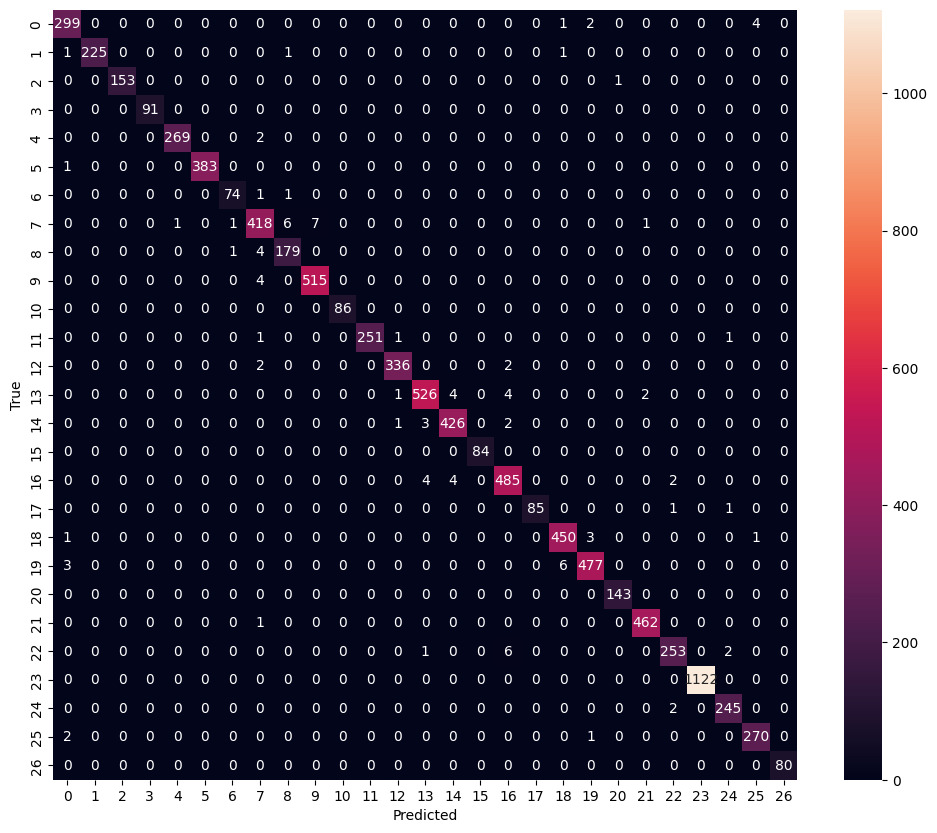
\includegraphics[width=0.6\textwidth]{confusion_matrix.jpg}
	\caption{Confusion matrix of CLIP model}
	\label{fig:confusionmatrix}
\end{figure}



\chapter{Conclusion}
\label{sec:conclusion}


% Include literature

\newpage
% References
%\printbibliography

\end{document}